
\chapter{Background \& Related Work}

% This chapter introduces the core concepts built upon in this thesis and surveys
% recent literature tackling the evaluation of generative graph neural networks (GNNs)
% and the relevance of this problem in structural biology. Section
% [\textbf{REVISE}] defines core mathematical and biological concepts that will
% be built upon in the thesis. Section [\textbf{REVISE}] will discuss recent
% advances in the design of measures used to evaluate generative GNNs and in
% structural biology.

This chapter introduces fundamental concepts built upon in this thesis, which
lies at the interface between structural biology and machine learning. First, we
start by defining some relevant biological properties of proteins, as well as
several representations leveraged in later chapters. We then introduce
generative models, applied to graphs and other domains. Crucially, we discuss in
detail the evaluation problem when it comes to generative models, as well as
some of the unique challenges arising in the graph domain specifically. Finally,
we discuss the current landscape of methods used to evaluate
graph generative models, such as the maximum mean discrepancy. Finally, we
introduce kernels can be used within the maximum mean discrepancy.

\section{Proteins}\label{sec:proteins}

Proteins are large biomolecules that are formed from a sequence of amino acids,
performing their functions as determined by their three-dimensional structure,
and amino acid sequence. Proteins support a vast array of functions in living
organisms, such as catalysing metabolic reactions, DNA replication, providing
structural support to cells, transporting molecules and sensing stimuli.

Each protein is made up of one or more chains of amino acids, and contain a
backbone and different side chains. The atoms in the backbone include a
\textalpha{}-carbon, another carbon and a nitrogen atom. An overview of the
peptide backbone is shown in Figure \ref{fig:backbone}. Interestingly, a plane
is forned by two alpha carbons, the carboxyl group, and the hydrogen atom
attached to the nitrogen atom (see Figure \ref{fig:backbone}), making the
peptide bond between the nitrogen and carbon atom resistant to twisting. That
means that the rotations enabling the 3D folding of a protein is governed by the
angle of the bonds linking the nitrogen atom to the \textalpha{}-carbon and the
other carbon atom to the \textalpha{}-carbon, named \textphi{} and \textpsi{}.
These angles' values are frequently used to validate proteins, characterise the
secondary structure of proteins (i.e. structural features observed in certain
segments of proteins), etc.


\begin{figure}[h]
  \centering
  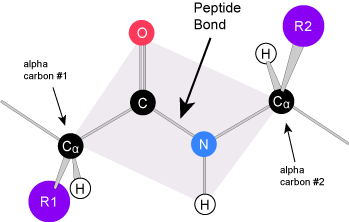
\includegraphics[width=.6\textwidth]{./figures/peptide_bond.png}
  \caption[Schematic of the backbone of a protein.]{Schematic of the backbone of a protein. Two \textalpha{}-carbons are
    shown as well as a \textbeta{}-carbon in the middle. R1 and R2 represent the
    side chains of the amino acid. }
  \label{fig:backbone}
\end{figure}


To visualize such angles, a Ramachandran plot can be constructed for any
protein. Such a plot can reveal secondary structural features such as
\textbeta{}-sheets, \textalpha{}-helices, etc. An example of such a plot together
with a 3D model of a protein can be found in Figure \ref{fig:ramachandran}.

\begin{figure}[h]
  \centering
  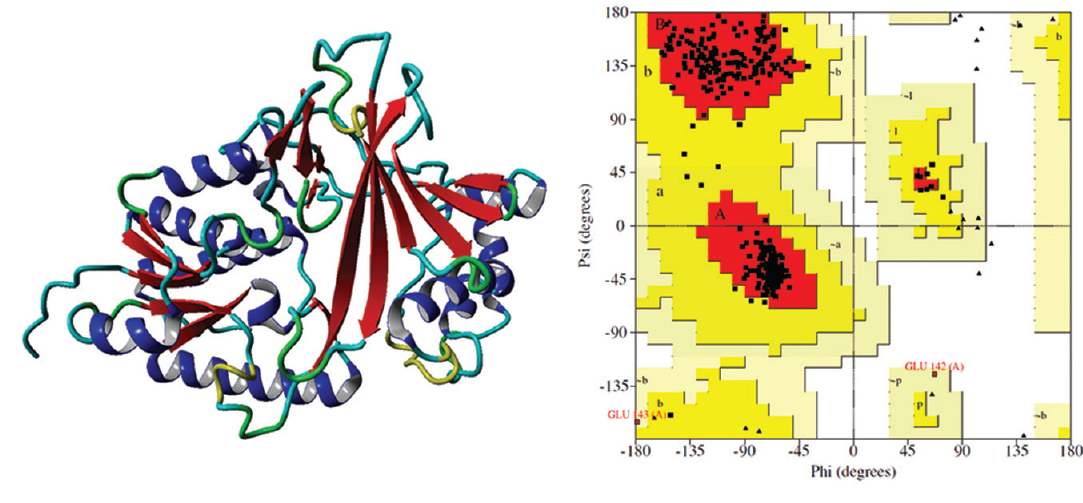
\includegraphics[width=.7\textwidth]{./figures/ramachandran_plot.jpg}
  \caption[3D structure of uridine diphosphogalactofuranose-galactopyranose
  mutase with a corresponding Ramachandran plot.]{3D structure of uridine diphosphogalactofuranose-galactopyranose
mutase with a corresponding Ramachandran plot. The \textalpha{}-helices can be
found on the middle left part of the Ramachandran plot, the \textbeta{} sheets on
the upper right quadrant, and the left handed \textalpha{}-helices can be found in
the middle upper right part of the plot. This figure is adapted from
\cite{nayak2018identification}.}
  \label{fig:ramachandran}
\end{figure}

\section{Graphs}\label{sec:graphs}

Proteins are often abstracted using graphs. A graph $G$ is a pair of vertices
$V$ and edges $E$ such that $G=(V, E)$, $|V|=n$ and $|E|=m$. Two vertices $i$
and $j$ are adjacent if there is an edge between them, i.e. $e_{ij}\in E$. The
relationship between between edges can be represented as an $n\times n$
adjacency matrix $A$, where:
\begin{equation}
  \label{eq:adjacency}
  A_{ij}=\begin{cases}
    1, \quad\text{if } e_{ij}\in E\\
    0, \quad\text{otherwise.}
  \end{cases}
\end{equation}
The neighborhood of a node $v$ is the set of nodes with an edge directly to $v$,
i.e. $N(v) = \{ u\in V|e_{uv} \in E \}$. A graph is undirected if the edges do
not contain directional information, i.e. $A_{ij}=A_{ji}$. A directed graph
would result in directionality being encoded in edges, where $A_{ij}$ would not
contain any information about $A_{ji}$. Nodes and edges in each graph can
contain one or more labels. In this thesis, we will mostly deal with labeled
undirected graphs, where each node will be labeled according to the amino acid
type each node belongs to.

There are multiple ways of constructing graphs from proteins. First, one can
extract a \emph{contact map} of a protein by computing the (euclidean) distance
between any two points belonging to each amino acid. The \textalpha-carbon is
often used for this purpose. This is a fully connected graph with continuously
labeled edges representing the distance between each node. From there, it is
possible to either extract a $k$-nearest neighbour ($k$-NN) graph, where
$k\in\mathbb{N}>0$ defines the amount of nodes directly connected to any given
nodes; or an $\varepsilon$-graph, where each node within a given distance
$\varepsilon\in\mathbb{R^+}\setminus \{0\}$ of another node is connected. Both
are graphs where each node is labeled with the residue name to which the
\textalpha{}-carbon belongs and the edges are unlabeled.

\section{Topological Data Analysis}\label{sec:tda}

Although graphs are powerful representation of proteins, the latter can also be
represented as \emph{point clouds}. One powerful field of study of topological
properties of point clouds (among other structured data) is \emph{topological
data analysis}.

Topology has witnessed relentless theoretical progress since Henri Poincar\'e
first addressed topological ideas as a distinct branch of mathematics in his
1895 publication of \textit{Analysis Situs}~\citep{poincare1895analysis}. Only
recently, -- with the advent of modern computing -- has the field of
computational topology and topological data analysis (TDA) gained momentum to
investigate (high-dimensional) data in physics, biology, and
beyond~\citep{dey1999computational, ghrist2008barcodes, amezquita2020shape}. For
material providing an extensive and formal introduction to topology and
persistent homology, please refer to~\citep{freedman2009algebraic,
edelsbrunner2010computational}, and \citep{ghrist2008barcodes}.

A powerful computational technique to analyse topological properties of point
clouds is \emph{persistent homology}, which first requires us to define
simplicial homology. Simplicial homology refers to a way of assigning
connectivity information to topological objects, such as point clouds, which are
represented by simplicial complexes. A simplicial complex $K$ is a set of
simplices which correspond to vertices in dimension 0, edges in dimension 1 and
triangles in dimension 2. The subsets of a simplex $\sigma\in K$ are referred to
as its faces, and every face $\tau\in K$. Moreover, any non-empty intersection
of two simplices also needs to be part of the simplicial complex, i.e.
$\sigma\cap\sigma '\neq\emptyset$ for $\sigma,\sigma '\in K$ implies
$\sigma\cap\sigma'\in K$, meaning that $K$ is closed under calculating the faces
of a simplex.

Persistent homology extends simplicial homology by employing filtrations to
imbue $K$ with scale information. This process captures rich, mutli-scale
topological information related to $K$ in a principled way. The filtration
process is generally defined by a function $f: K\to\mathbb{R}$ satisfying some
finite number of values $m$ and $f^{0}\leq f^{1}\leq\dots\leq f^{m-1}\leq
f^{m}$. This allows us to sort $K$ using $f$, for instance by extending $f$
linearly to higher-dimensional simplices via $f(\sigma):=\max_{v\in\sigma}f(v)$,
leading to a nested sequence of simplicial complexes like so:
\begin{equation}
  \label{eq:nested_simplicial_complexes}
  \emptyset=K^{(0)}\subseteq K^{(1)}\subseteq \dots\subseteq K^{(m-1)}\subseteq K^{(m)},
\end{equation}
where $K^{(i)}:=\{\sigma\in K\ |\ f(\sigma)\leq f^{(i)}\}$. This relationship
enables tracking the appearance (i.e. a connected component arising) and the
dissapearance (i.e. two connected components into one) of topological features
across scales as one transitions from $K^{(i)}$ to $K^{(i+1)}$. The birth (i.e.
appearance) and death (i.e. dissapearance) of topological features for different
values of $f$ are usually summarized in a \emph{persistence diagram}, which is a
multiset of tuples, each of which contains the values at which each features is
born or dies.

A common construction for obtaining such features is the Vietoris-Rips complex
\citep{vietoris1927hoheren}. It requires a distance threshold $\varepsilon$ and
a metric $\d( \cdot, \cdot)$ (usually, the Euclidean distance, as we will
use in this thesis). The Vietoris-Rips complex at scale $\varepsilon$ of an
input protein point cloud is defined as
$\mathcal{V}_{\varepsilon}(X):=\{\sigma\subseteq X| \d(x(i),
x(j))\leq\varepsilon\},\ \forall x(i),x(j)\in\sigma$, i.e.
$\mathcal{V}_{\varepsilon}$ contains all subsets of the input space whose
pairwise distances are less than or equal to $\varepsilon$.
$\mathcal{V}_{\varepsilon}$ is conceptually very similar to the
$\varepsilon$-graphs discussed in section \ref{sec:graphs}, except that
$\varepsilon$ here ranges over the entire space of possible distance values, and
$\mathcal{V}_{\epsilon}$ also tracks topological features over all three
dimensions, instead of only connected nodes.

Note that the multiplicity of the persistence diagram corresponds to the number
of homology dimensions under study. In this thesis, given proteins are
represented as three-dimensional point clouds, we choose to track topological
features across three homology dimension: 0,1 and 2. Effectively, this tracks
connected components in dimension 0, circular holes in dimension 1 and two
dimensional voids or cavities in dimension 2 as the filtration function is
applied. For a more thorough introduction to homology and homology groups,
please refer to \cite{edelsbrunner2010computational}.

\section{Generative models}\label{genmodels}

This thesis deals with measures to assess generative model performance, so we
define generative models here. While discriminative machine learning techniques
aim to learn some dependent variable $\mathcal{Y}$ from a set of (independent)
features $\mathcal{X}$, generative machine learning models generate synthetic
samples $\mathcal{X}'$ following the distribution of $\mathcal{X}$. Computing
such probabilistic distributions through maximum likelihood estimation and
related methods is intractable in many cases; as such, new learning paradigms
were established to enable the modeling of complex, real-world distributions
through gradient-based methods.

One such seminal method was that of generative adversarial learning, pioneered
by \cite{goodfellow2014generative}, where a (deep) generator is pitted against
a (deep) discriminator. The former's goal is to generate samples identical to
the training distribution, while the latter is to classify whether or not the
sample originated from the generator or the training distribution.
Simultaneously developed methods by \cite{kingma2013auto} generalized this idea
further and introduced the variational auto-encoder, where instead of a
discriminator, the second network leverages the representation of the generator
to perform approximate inference. In both cases, the two networks (i.e. the
generator and the discriminator/inference network) are jointly trained using
backpropagation to minimize some appropriate loss function.

A recent review of the existing landscape of generative modelling methods has
been provided by \cite{bond2021deep}.

These techniques have been particularly successful in the image domain, where
modern GANs have been able to tackle multiple practical challenges such as mode
collapse and convergence failure to produce realistic images, such as the sample
seen in Figure \ref{fig:styleganxl}. More pertinent to this thesis is the
application of generative models to graphs. The application domain has been
reviewed by \cite{zhou2020graph}. In short, graph generative networks are
capable of operating on the highly versatile and extensible graph domain. It has
been shown that they can produce small molecules, generate social networks,
knowledge graphs, among many other real-world tasks. Generative networks can be
grouped into two categories: those that generate nodes in each graph
sequentially, such as GraphRNN by \cite{you2018graphrnn}, and those that generate
graphs from some latent distribution directly, such as MolGAN by
\cite{de2018molgan}.

\begin{figure}
  \centering
  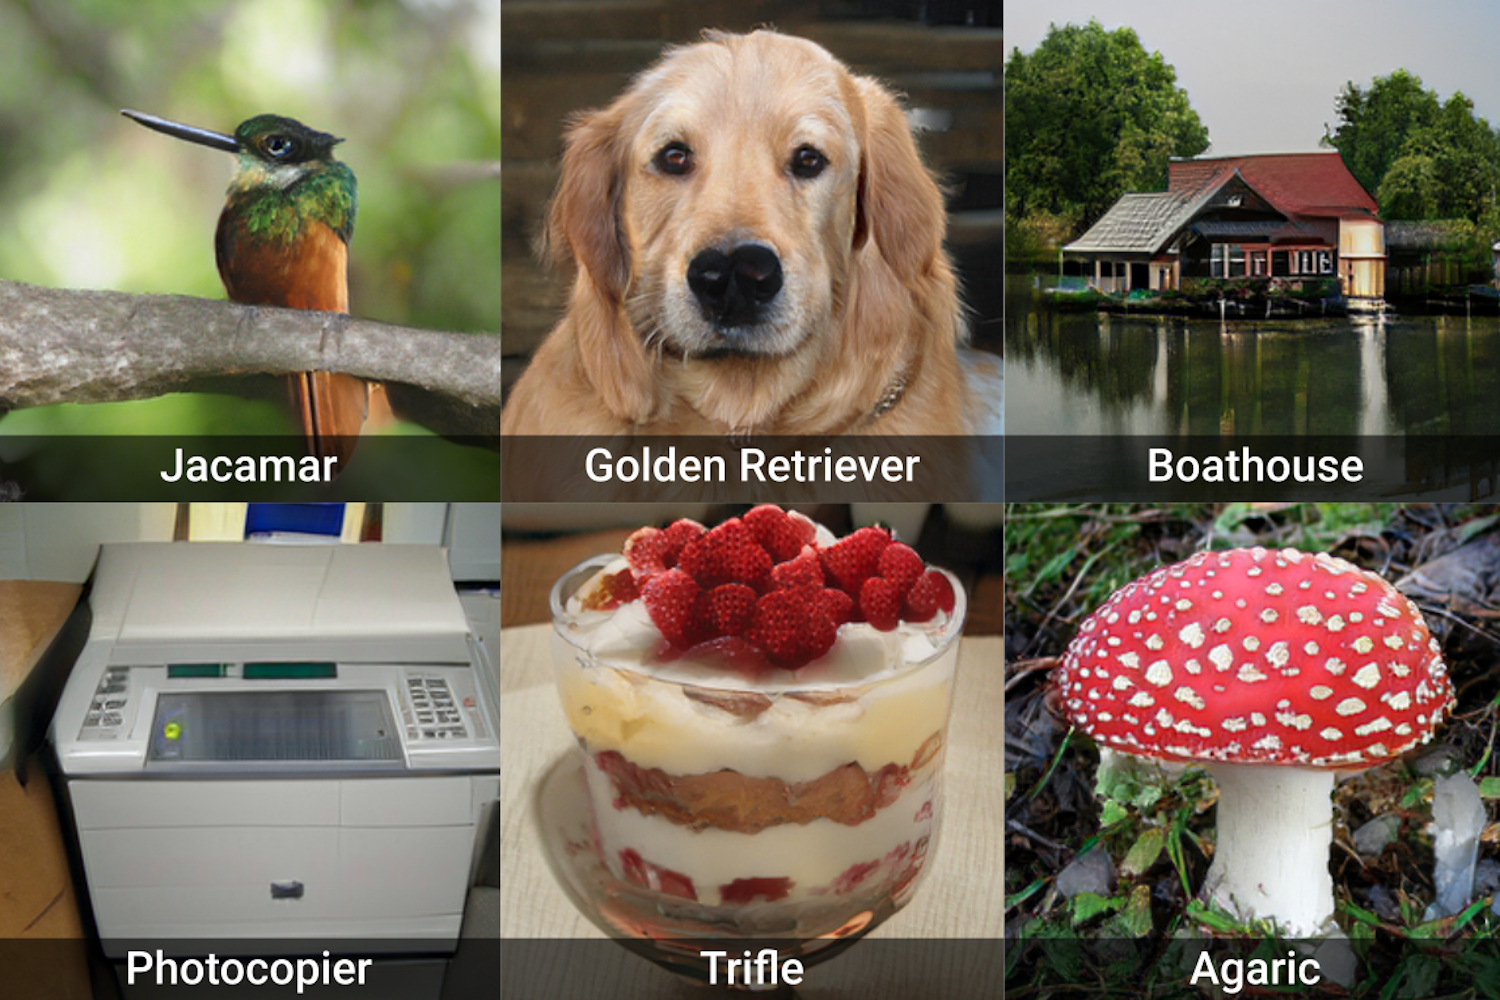
\includegraphics[width=0.45\textwidth]{./figures/representative_image.jpg}
  \caption[Sample images generated by StyleGAN-XL]{Sample images generated by StyleGAN-XL, the state-of-the-art GAN
by \cite{sauer2022stylegan} at the time of writing.}
  \label{fig:styleganxl}
\end{figure}

Operating in the graph domain incurs some unique challenges. From a modelling
standpoint, dealing with graphs means dealing with a much larger and variable
output space. In the general case, at least $n^2$ values need to be specified.
Additionally, the number of edges and nodes vary from sample to sample, which
also needs to be accounted for in the model structure. Additionally, building a
generative model generating graphs of up to $n$ nodes, $n!$ possible adjacency
matrices can be generated. Such a high representation complexity is challenging
to model, expensive to compute, and difficult for objective functions to
optimize. The last modelling-related issue when dealing with graphs is that the
presence of one edge is not independent from another, i.e. real-world graphs
often exhibit patterns of local connectedness which need to be accounted for in
the model.

\section{The Evaluation Problem}\label{sec:evalproblem}

But perhaps the most significant problem plaguing all generative models is the
evaluation problem. Concretely, this problem can be framed using the following
question: how does the practitioner go about evaluating the quality of the set
of samples generated? While sidestepping the problem is possible in the image
domain by manually inspecting generated samples, a practice that might reveal
interesting modelling pathologies (see Figure \ref{fig:ganpathologies}), this
cannot be done at scale, nor can it be done for generative models operating in
the graph domain, where human perception cannot easily evaluate the quality of a
set of generated graphs. The community has therefore devised a set of measures
to attempt to rank models more adequately.

\begin{figure}
  \centering
  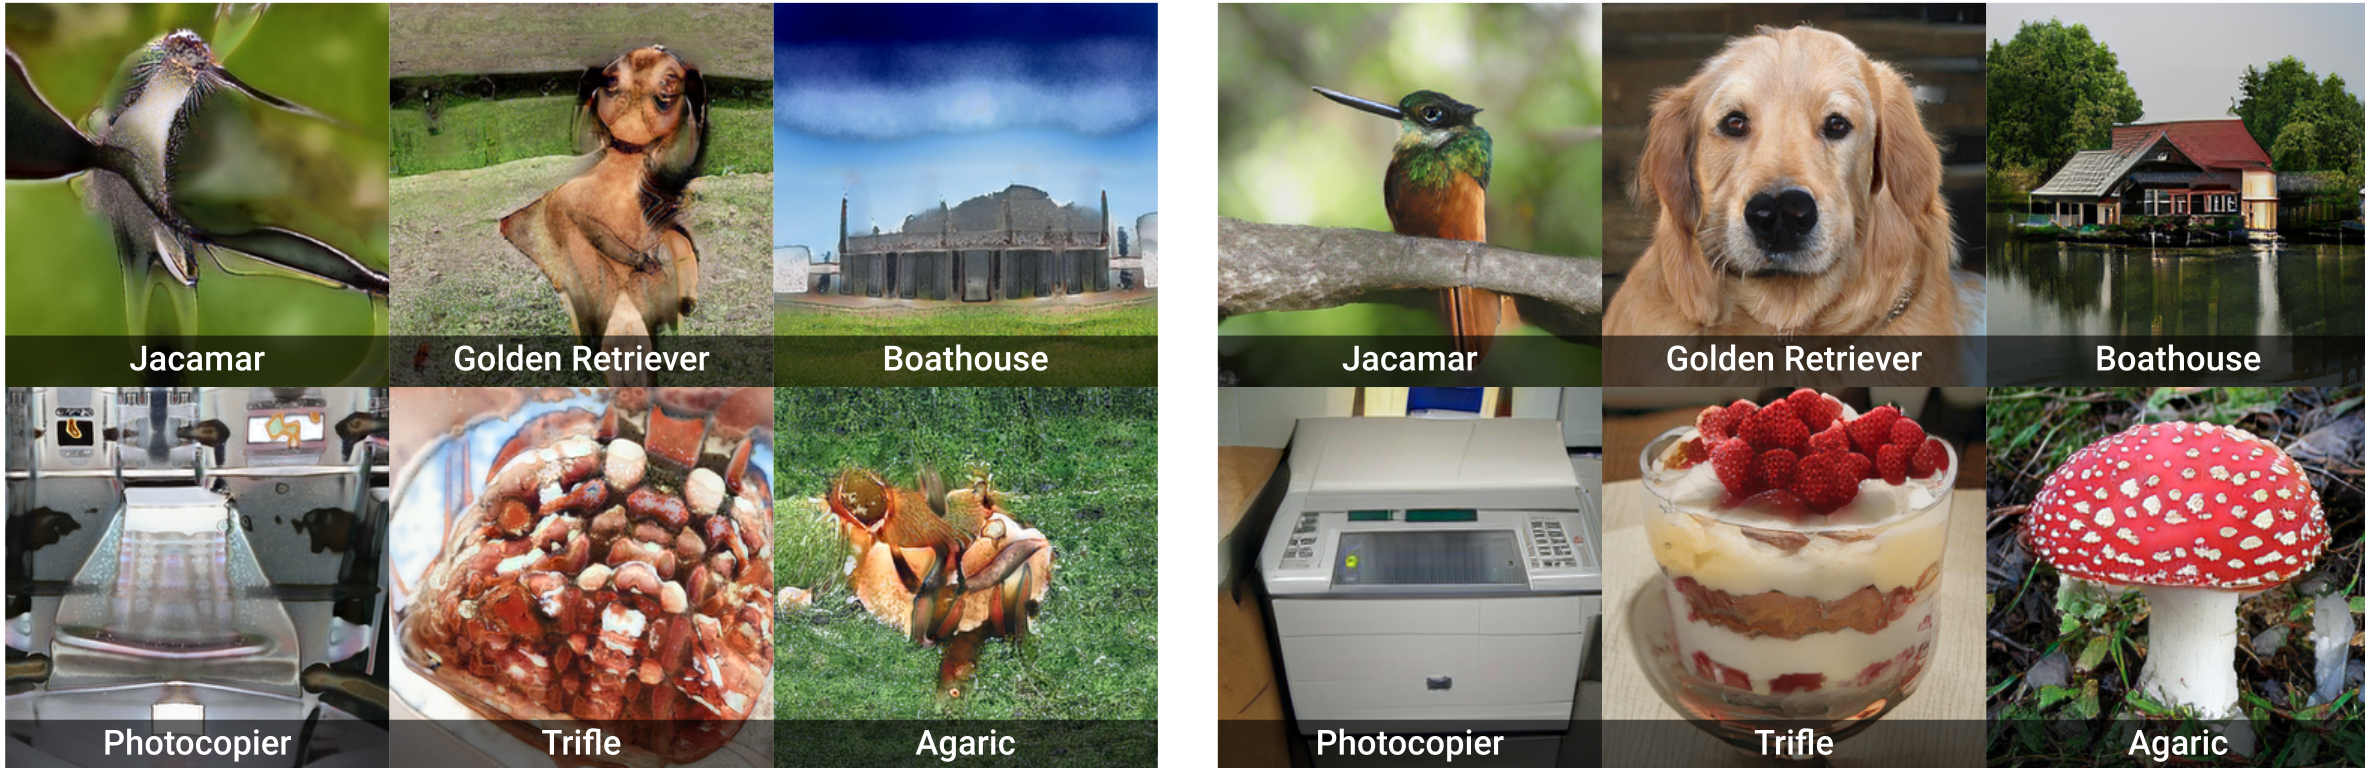
\includegraphics[width=\textwidth]{figures/pathologies.png}
  \caption[Class-conditional samples from StyleGAN3 and
  StyleGAN-XL]{Class-conditional samples generated by StyleGAN3 (left) and
    StyleGAN-XL (right) trained on the same dataset at the same resolution. This
    figure is adapted from \cite{sauer2022stylegan}.}
  \label{fig:ganpathologies}
\end{figure}

Before going through existing metrics, it is useful to state broad goals, or
\emph{desiderata} of metrics concerning generative modelling. As highlighted by
\cite{o2021evaluation}, (pseudo)-metrics must be endowed with the following
properties:

\begin{enumerate}
\item \textbf{Expressivity}: Given two sets of samples $\mathcal{X}_1$ and
$\mathcal{X}_2$, a suitable measure $\td$ should have
$\td(\mathcal{X}_1,\mathcal{X}_2)$ increasing monotonically as
$\mathcal{X}_1$ and $\mathcal{X}_2$ become more and more dissimilar.
\item \textbf{Robustness}: $\td(\mathcal{X}_1,\mathcal{X}_2)$ should be
robust to small perturbations in either sets.
\item \textbf{Efficiency}: $\td(\mathcal{X}_1,\mathcal{X}_2)$ should be
fast to calculate should scale well with size and number of graphs.
\end{enumerate}


For images, an interesting metric (and the current standard for that domain) is
the Fr\'echet Inception Score, as introduced by \cite{heusel2017gans}. Overall,
the goal of this metric is to calculate some distance between the activations of
a neural network feature computed from both the real-world images the network
was trained on and the synthesized images. Concretely, this is achieved by
calculating the squared Wasserstein metric between the generated and real
representations computed from a neural neural network (commonly, the Inception
v3 architecture from \cite{szegedy2015rethinking} is used) as two
multidimensional Gaussian distributions with parameters $\mathcal{N}(\mu,
\Sigma)$ and $\mathcal{N}(\mu_{rw}, \Sigma_{rw})$, respectively. The general
formulation of the $p$\textsuperscript{th} Wasserstein distance between two
distributions $u$ and $v$ is given by

\begin{equation}
  \label{eq:wasserstein_distance} W_p(u,v) := \left(\inf _{\gamma \in \Gamma
(u,v)}\int _{M\times M}d(x,y)^{p}\,\mathrm {d} \gamma (x,y)\right)^{1/p},
\end{equation}

where $(M, d)$ is a metric space, $\Gamma (u,v)$ denotes the collection of all
measures on $M\times M$ with marginals $u$ and $v$ on the first and second
factors, respectively. Intuitively, $W_p(u,v)$ can be interpreted as a
generalization of the Minkowski distance between probability distributions
instead of fixed-length vectors, the latter being given by:

\begin{equation}
  \label{eq:minkoski}
  d\left(X,Y\right)=\left(\sum _{i=1}^{n}|x_{i}-y_{i}|^{p}\right)^{\frac {1}{p}}.
\end{equation}

In the case of the Fr\'echet Inception Score, the squared Wasserstein distance
between the Inception v3-derived representations of the images can be
reformulated as follows:
\begin{equation}
  \label{eq:fid}
  \text{FID}=||\mu -\mu _{rw}||_{2}^{2}+\operatorname {tr} (\Sigma +\Sigma
_{rw}-2(\Sigma ^{1/2}\Sigma _{rw}\Sigma ^{1/2})^{1/2}).
\end{equation}

For the graph domain, such a measure is unfeasible due to the varying size of
the output graphs and the lack of common consensus on embedding methods, partly
due to the diversity of graph types, although progress is being made on this
front, as reviewed by \cite{xu2021understanding}. Interesting strides have been
made in some domains, such as in the drug discovery field, where the penultimate
layer of the ChemNet neural network can be used as input to the FID as showed by
\cite{preuer2018frechet}.

However, an interesting approach recently explored by
\cite{thompson2022evaluation} leverages the observation, made in part by
\cite{xu2018powerful,morris2019weisfeiler}, and \cite{kipf2016semi}, that
certain GNNs have the ability to extract meaningful
representations without any training. Through a set of two perturbation
experiments, similar to the work done by \cite{xu2018empirical} and
\cite{o2021evaluation}, \cite{thompson2022evaluation} show that using a
randomly initialized Graph Isormorphism Network (GINs), first introduced by
\cite{xu2018powerful}, provides a strong, domain-agnostic metric to evaluate
generative GNNs. GINs --like the majority of GNNs for discriminative machine
learning purposes-- consist in (i) $L$ propagation layers that perform some form
of message passing between the nodes, computing rich representations of each
node's neighbourhoods and (ii) some readout layer, aiming to compute some
embedding and subsequent output. For GINs, the message passing layers computing
each (hidden) node embedding $v$ at layer $l$ (denoted $\mathbf{h}_{v}^{(l)}$)
is assigned the following value:
\begin{equation}
  \label{eq:mplgin}
  \mathbf{h}_{v}^{(l)}:=\text{MLP}^{(l)}\left(\mathbf{h}_{v}^{(l-1)} +
f^{(l)}\left(\left\{ \mathbf{h}_{v}^{(l-1)}: u\in N(v)\right\}\right)\right),
\end{equation}

$\forall v\in V$ where $V$ is as defined in section \ref{sec:graphs},
$\forall\ l>0, \mathbf{h}_{v}^{(l)}\in\mathbb{R}^d$, $\text{MLP}^{(l)}$ is a
multilayer perceptron, and $f^{(l)}$ is some aggregating function, such as mean,
max or sum. The second part, i.e. the graph readout layer with skip connections,
aggregates features from all nodes at each layer $l\in [1,L]$, concatenating
them into one $(L\times d)$ dimensional vector $x_i$ as follows:
\begin{equation}
  \label{eq:readout_gin}
  \mathbf{x}_i = \text{CONCAT}\left(  g\left( \left\{ \mathbf{h}_{v}^{(l)} |\ v\in V \right\} \right) |\ l \in [1, L] \right)
\end{equation}

where $g$ can be chosen from the same set of functions as $f^{(l)}$. \textbf{[]}

While these developments are encouraging, practitioners designing generative
GNNs such as \cite{liao2019efficient, niu2020permutation}, and
\cite{you2018graphrnn} have generally gravitated towards the maximum mean
discrepancy (MMD) measure to evaluate the quality of the graph.

\section{Maximum Mean Discrepancy}\label{sec:mmd}

A significant part of this thesis is centered around investigating the MMD
statistic, so we define and examine existing around MMD research here. Introduced by
\cite{borgwardt2006integrating} and further exposited by
\cite{gretton2012kernel}, this measures leverages the expressive power and
versatility of \emph{kernel functions} to evaluate distances between two sample
distributions. What's more, \cite{gretton2012kernel} describe how this measure
can be treated as a test statistic, from which a $p$-value can be computed, to
test if two distributions are statistically significantly different from one
another. MMD is therefore an ideal platform to leverage when trying to assess
generative models.

First, we define \emph{kernels}, an essential component of MMD. They measure the
similarity of two sets of any structured object. Let $\mathcal{X}$ be a
non-empty set, and a \emph{kernel function}
$\tk:\mathcal{X}\times \mathcal{X}\to\R $ satisfying the following
properties:

\begin{itemize}
\item $\tk(x_i,x_j)=\tk(x_j,x_i)\ \forall\ x_i,x_j\in\mathcal{X}$
\item $\sum_{i,j}c_i,c_j\tk(x_i,x_j)\geq 0\ \forall\ x_i,x_j\in\mathcal{X},
  \forall\ c_i,c_j\in\R$.
\end{itemize}

Given $n$ samples from $\bx=\{x_1,\dots, x_n\}\subseteq\mathcal{X}$ and $m$
samples from $\by=\{y_1,\dots, y_m\}\subseteq\mathcal{X}$, the biased estimate
of $\MMD^2$ is given by:

\begin{equation}
  \label{eq:mmd}
  \MMD^2(X,Y) := {1\over n^2}\sum_{i,j=1}^n\tk(x_i, x_j) + {1\over m^2}\sum_{i,j=1}^m\tk(y_i,y_j) - {2\over nm}\sum_{i=1}^{n}\sum_{j=1}^{m}\tk (x_i,y_j)
\end{equation}

In accordance with Lemma 6 of \cite{gretton2012kernel}, the diagonal elements of
the first two kernel matrices in Equation \ref{eq:mmd} can be set to $0$ to
obtain an unbiased estimate of $\MMD$.

In the graph domain, it is now incumbent upon the practitioner to (i) choose an
appropriate (optional) graph descriptor and (ii) kernel with (iii) appropriate
kernel hyperparameters. This process, along with its pitfalls and current
practices, are discussed in more detail by \cite{o2021evaluation}, but we want
to give an overview of possible, common, and sensible choices for descriptor,
kernel, and hyperparameter.

A common practice in the literature is to first extract some fixed-length graph
representation using a range of commonly used descriptors such as:
\begin{itemize}
\item \textbf{The degree histogram.} Given a graph $G=(E,V)$ as defined in Section
  \ref{sec:graphs}, we can calculate $\deg(v)\forall v\in V$, where
  position $i$ of the resulting histogram is the number of vertices with degree
  $i$. With a given maximum $d$, we obtain a mapping $f:G\mapsto\R^d$. We will
  normalize the entries of the histogram to obtain a size-invariant descriptor.

\item \textbf{The clustering coefficient histogram.} The clustering
  coefficient of a vertex $v$ is defined as the fraction of edges within its
  neighborhood divided by the number of edges between neighbors, i.e.
  \begin{equation}
    C(v) := \frac{2\mleft|\mleft\{(v_i, v_j) \in E \mid  v_i \in N(v) \lor v_j \in N(v) \mright\}\mright|}{\deg(v) \mleft(\deg(v) - 1\mright)}.
  \end{equation}
  $C(v)\in\left[ 0,1 \right]$ measures the extent to which each vertex $v$ forms
  a clique \citep{watts1998collective}. The collection of coefficients can be
  captured for each graph in a histogram, which is also normalized.

\item \textbf{The Laplacian spectrum histogram.} The normalized graph Laplacian
  is given by $\laplace :=I-D^{-{1\over 2}}AD^{-{1\over 2}}$ where $A$ is the
  adjacency matrix (see Section \ref{sec:graphs}), $I$ the identity
  matrix and $D$ the degree matrix, where $D_{ii}=\deg(v_i)$ and $D_{ij}=0,
  i\neq j$. Since $A$ is symmetric (all graphs in this thesis are undirected),
  and that $\laplace$ is real-valued, it is also diagnonalizable, with
  eigenvalues $\eig_1\leq\eig_2\leq\ldots\forall\eig\in \left[0,2\right]$ -- see
  \cite{chung1997spectral}, 1997, Chapter 1, Lemma 1.7 for a proof of the boundedness. This lends
  itself again to some bounded, normalized histogram representation. As
  discussed by \cite{o2021evaluation}, it is unknown if graphs can be fully
  determined by their spectrum, and we know that for certain classes of graphs
  this is not the case \citep{schwenk1973almost}.

\end{itemize}

Of note, none of those three descriptors take node labels into account. This is
why we are going to investigate alternative kernels leveraging node labels (see
Section \ref{sec:kernels}), as well as use fixed-length vectors derived from
powerful transformer-based protein language models, specifically from the
Evolutionary Scale Modeling family \citep{rives10biological}. This family of
models allows us to obtain an embedding vector $h\in\R^d$ for each residue,
which we can then average to obtain one protein-level embedding by taking the
average across residues. Because transformers don't constitute an essential part
of this thesis, we redirect the reader to the original publication describing it
by \cite{vaswani2017attention}, as well as the excellent explainer by
\cite{alammar2018} for a fundamental discussion of the topic.

\section{Kernels}\label{sec:kernels}

Once graph representations are computed, it is possible to compute a kernel
between any two such vectorized representations using kernels. In this thesis,
we will use:

\begin{itemize}
\item The linear kernel. Let $\bx,\by\subseteq \mathcal{X}\in\R^d$, where $d$
  denotes the dimensionality of the graph descriptor (e.g. the number of bins in
  the clustering histogram). Then, the linear kernel is defined as:
  \begin{equation}
    \label{eq:linear_kernel}
    \tk(\bx, \by) = \bx^T \by + c
  \end{equation}
  with $c\in\R$.
\item The Gaussian kernel, which is given by:
  \begin{equation}
    \label{eq:gaussian_kernel}
    \tk(\bx, \by) = \exp\left( -{\lVert \bx-\by \rVert^2\over 2\sigma^2} \right)
  \end{equation}
\end{itemize}

We will neglect certain kernels used in the literature, either because they are not
positive semi-definite, such as the total variation kernel (see
\cite{o2021evaluation}, Appendix A1 for a proof), or because they bring capture
little more information compared to existing accepted alternatives, they are
inefficient to compute and not recommended to evaluate generative GNNs, e.g. the
Earth mover's distance-based kernel \citep{o2021evaluation}.

We will, however, leverage two new classes of kernels that are applicable to
models evaluating protein generative model performance. The first are graph
kernels (reviewed by \cite{borgwardt2020graph}). In particular we will examine
an efficient and expressive kernel used for biological
data: the Weisfeiler-Lehmann kernel. The second class of kernels leveraged here
operate directly on the persistence diagrams obtained using the filtration
procedures described in section \ref{sec:tda}, in particular the
persistence Fisher kernel introduced by \cite{le2018persistence}. We define both
in the next paragraphs.

\paragraph{The Weisfeiler-Lehmann algorithm} Originally designed as a graph
isomorphism test by \cite{weisfeiler1968reduction}, the eponymous
algorithm provides a powerful and computationally efficient way of capturing
local node neighborhood information to quantify the degree of similarity between
any two graphs, which works for both labeled and unlabeled graphs. The capturing
of local neighborhood information is achieved by relabelling each node based on
the hashed value obtained from concatenating the node label of each neighbour
$h$ times. The degree of each node can be used when dealing with unlabeled
graphs. In this thesis, however, the amino acid type will be used as a node
label. An example of a Weisfeiler-Lehman procedure can be seen in Figure
\ref{fig:wl_algo}. A kernel can be computed between two graphs by computing the
dot product of two resulting hash histograms obtained at the end of the
Weisfeiler-Lehman algorithm \citep{shervashidze2011weisfeiler}.

\begin{figure}
  \centering
  \begin{subfigure}[b]{0.49\textwidth}
    \centering
    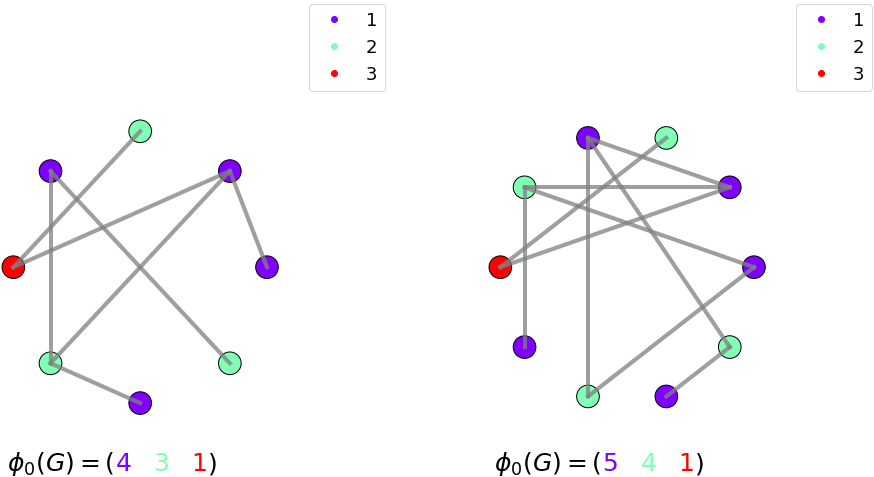
\includegraphics[width=\textwidth]{./figures/WL/WL1.png}
    \caption{First iteration of the Weisfeiler-Lehman algorithm.}
  \end{subfigure}
  \hfill
  \begin{subfigure}[b]{0.49\textwidth}
    \centering
    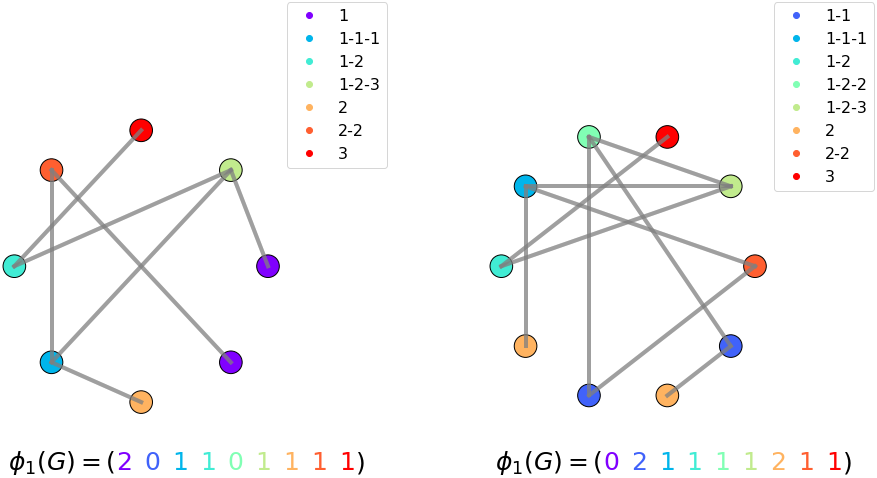
\includegraphics[width=\textwidth]{./figures/WL/WL2.png}
    \caption{Second iteration of the Weisfeiler-Lehman algorithm.}
  \end{subfigure}
  \par\bigskip
  \begin{subfigure}[b]{0.5\textwidth}
    \centering
    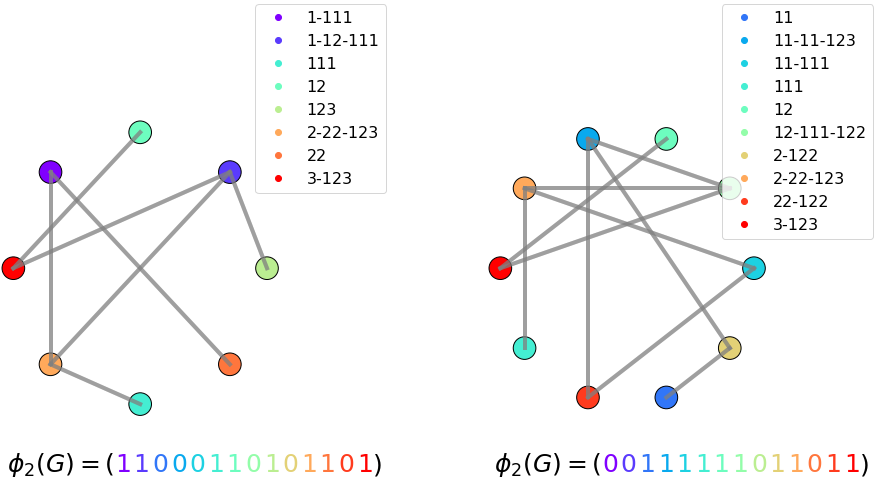
\includegraphics[width=\textwidth]{./figures/WL/WL3.png}
    \captionsetup{width=1.4\linewidth}
    \caption{Third iteration of the Weisfeiler-Lehman algorithm.}
  \end{subfigure}
  \caption[Three iterations of the Weisfeiler-Lehman algorithm.]{Three iterations of the Weisfeiler-Lehman node relabelling algorithm.
    The kernel between the two graphs can be computed by computing
    $k_{WL}(G,G')=\phi_2(G)\cdot\phi_2(G')$. Imagery adapted from \cite{mengin2019}.}
  \label{fig:wl_algo}
\end{figure}

\paragraph{Persistence diagram kernels} Kernels between persistence diagrams
also offer powerful similarity measures between the global shape of proteins using the
persistence diagrams produced by the Vietoris-Rips filtration, thereby going
beyond just looking at the neighbourhoods of each node in the case of the
Weisfeiler-Lehman procedure described above.

We first look at the Persistence Fisher kernel, introduced by
\cite{le2018persistence}. Given two diagrams $\dgi$ and $\dgj$, the Persistence
Fisher kernel $k_{PF}$ is given by:
\begin{equation}
  \label{eq:kpf}
  k_{\text{PF}}(\dgi, \dgj ) :=\exp\left(-td_\FIM(\dgi,\dgj)\right)
\end{equation}

where:
\begin{equation}
  \label{eq:dfim}
  d_\FIM(\dgi, \dgj) := d_{\calp} \! \left(\rho_{\left(\dgi \cup \text{Dg}_{j\Delta}\right)}, \rho_{\left(\dgj \cup \text{Dg}_{j\Delta}\right)} \right),
\end{equation}

and

\begin{equation}\label{equ:dFIM}
  d_{\calp}(\rho_i, \rho_j) = \arccos \! \left(\int \!\!\sqrt{\rho_i(x) \rho_j(x)} \mathrm{d}x \right).
\end{equation}

is defined as the Fisher Information Metric, with $\rho_i$ and  $\rho_j$ being
two persistence diagrams which can be represented as points in a probability
simplex $\bbp := \left\{ \rho|\int\rho(x)\d x=1,\rho(x)\geq 0\right\}$. Indeed,
considering persistence diagrams as points can be achieved by setting:
\begin{equation}
  \label{eq:pdsaspoints}
  \rho_{\dg} := \left[ {1\over Z} \sum_{u\in\dg}\caln(x;u,\sigma I)\right]_{x\in\Theta}
\end{equation}

where $Z=\int_{\Theta}\sum_{u\in\dg}\caln(x;u,\sigma I) \mathrm{d} x$, $\caln$ is a
Gaussian distribution, $I$ the identity matrix, and $\sigma>0$ is the smoothing
parameter is chosen by the practitioner. Note that if the set $\Theta$ is set to
the Euclidean space, as will be the case in this thesis, each persistence
diagram then turns to a probability distribution, which is what allows us to
compute the Fisher information metric
\citep{anirudh2016riemannian,adams2017persistence}.

\section{Summary}

In this section we introduced fundamental characteristics of proteins by
first discussing how amino acids form a backbone and each of them forms two dihedral
angles with their neighbour to make up the three-dimensional structure of the
protein. We then showed how one can represent proteins using graphs, either by
using $k$-nn graphs or $\varepsilon$-graphs. We explored an alternative
representation strategy using topological data analysis and discussed how it
allows one to capture global structural features of the protein.

We then moved on to introduce generative models, and discuss recent advances in
such models in the image domain, where such models were first developed. We then
proceed to discuss generative models in the graph domain, along with the unique
computational challenges that it incurs from a modelling standpoint.
Importantly, we outline the evaluation problem arising when evaluating
generative networks, specifically in the graph domain, and outline the
desiderata for good metrics: expressivity, robustness and efficiency. We examine
current accepted practices and introduce the maximum mean discrepancy, the main
method used in this thesis. We finally introduce the collection of kernels that
we are going to leverage using the maximum mean discrepancy.
